\lecture{Thu. 9/20/12}

Problem set 2 is out.

Last time we talked about CFG's, CFL's, and PDA's. Today we will talk about
\begin{itemize}
\item
CFG$\to $PDA,
\item
non-CFL's
\item
Turing machines
\end{itemize}

Recall what nondeterminism means: every time there are multiple possibilities, the whole machine splits into independent parts. As long as one thread lands in an accept state, then we accept.
Nondeterminism is a kind of guessing and checking that the guess is correct.

When we define the model for a PDA, the PDA can pop something from the stack. There is no hardware (bulit-in function) to test if the stack is empty, but we can use ``software" (i.e. clever programming) to test if the stack is empty: to start off, write a $\$$, and when the machine sees $\$$, it knows that the stack is empty. Thus we can allow any PDA to test whether the stack is empty. We'll use this in many of our examples.

To jog your memory, a CFG is made up of a set of rules like the following:
\bal
E&\to E+T|T\\
T&\to T\times F|F\\
T&\to (E)|a.
\end{align*}
We saw that this CFG recognizes $a\times a+a$: we had a derivation of $a\times a\to a$ given by
\[
E\implies E+T\implies T+T\implies T+F\implies\cdots \implies a\times a+a.
\]
\subsection{CFG's and PDA's recognize the same language}
Our main theorem of today is the following.
\begin{thm}
$A$ is a CFL iff some PDA recognizes $A$.
\end{thm}
In other words, CFG's and PDA's have exactly the same computing power; they generate the same class of languages. To prove this we'll simulate one kind of computation with another kind of computation.
\begin{proof}
We need to prove
\begin{enumerate}
\item
CFG$\to$PDA (we'll do this today)
\item
PDA$\to$CFG (skip, see the book. This is more technical.) %``programming" is easier)
\end{enumerate}
\end{proof}
%You don't need to know the proof of the second item 
\begin{cor}
\begin{enumerate}
\item
Every regular language is a CFL.
\item
The intersection of a context-free language and a regular language is a context-free language.
\[
\text{CFL }\cap\text{ regular}=\text{CFL}. 
\]
\end{enumerate}
\end{cor}
\begin{proof}
\begin{enumerate}
\item
A finite automaton is a pushdown automaton that just doesn't use the stack.
\item  Omitted. (See Exercise 2.18a in the book---basically just take the states to be the product set.)
\end{enumerate}•
\end{proof}
Note 2 is weaker than the statement that the intersection of two context-free languages is a context-free language, which is not true.
\begin{pr}
The intersection of two CFL's, or the complement of a CFL, is closed under $\cup,\circ,*$, but not under $\cap$ or complementation.
\end{pr}
\begin{proof}
Just give a construction using grammars or pushdown automata.
\end{proof}
\subsection{Converting CFG$\to$PDA}
\begin{proof}[Proof sketch]
We convert a CFG into a PDA. %The idea is the following.

The input is a string that may or may not be in the language; our PDA has to say whether it is.

Recall that the derivation is the sequence of strings we go through to get to a string in the language. {\it We use nondeterminism to guess the derivation.}

We first write down the start variable on the top of the stack. Take whatever string is written down on the stack to be the current working string. Take one of the variables on the stack and in the next step, replace it using one of the rules. There may be several possible steps; we consider all possibilities using nondeterminism.

%For every derivation we can preferentially do the one on the left first. For instance, for $a\times a+a$, we can do $E\implies E+T\implies T+T\implies F+T\implies \cdots $

For instance, we'd want the machine to operate as follows.

\begin{center}
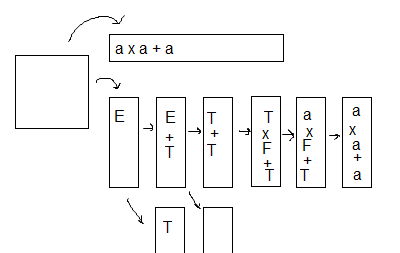
\includegraphics{5-1}
\end{center}

At the end we pop the symbols and compare with the input string, and then test the stack for emptiness at the end.

However, there's a problem: what if we want to replace some symbol {\it not} at the top?
The idea is the following: if the top of the stack has a terminal symbol (which can't be replaced by anything), let's match it against the next symbol in the input word immediately. %If we can't match it, this branch of the nondeterminism just fails. 
Whenever we have a terminal symbol at the top of the stack, we pop and compare until a variable (such a F) is at the top. Sooner or later, we'll have a variable at the top, and then we can try one of the substitutions. 

See the textbook for details.
\end{proof}
\subsection{Non-CFLs}
CFG's are powerful but there are still many languages they can't recognize!

We will show the language
\[
\set{a^kb^kc^k}{k\ge 0}
\]
is not a CFL. Note by contrast that $\set{a^kb^k}{k\ge 0}$ is a CFL (Example~\ref{ex:akbk}).

An intuitive argument is the following: we can push the $a$'s, compare with the $b$'s by popping the $a$'s, but when we get to the $c$'s we're out of luck: the $a$'s were all popped off, and the system has not remembered any information about the $a$'s. However, as we've said, we have to be careful with any argument that says ``I can't think of a way; thus it can't be done." How do you know the machine doesn't proceed in some other tricky way?

By contrast, if we look at the strings $a^kb^lc^m$ where either the number of $a$'s equal the number of $b$'s, {\it or} the number of $a$'s equal the number of $c$'s, this can be done with pushdown automaton. (Use nondeterminism, left as exercise.)

We'll give a technique to show that a language is not a CFL, a pumping lemma in the spirit of the pumping lemma for regular languages, changed to make it apply to CFL's.

Our notion of pumping is different. It is the same general notion: all long strings can be ``pumped" up and stay in the language. However, we'll have to cut our string into 5 rather then 3 parts.

\begin{lem}[Pumping lemma for CFL's]\llabel{lem:pump-cfl}
For a CFL $A$, there is a pumping length $p$ where if $s\in A$ and $|s|\ge p$, then $s$ can be broken up into $s=uvxyz$ such that
\begin{enumerate}
\item
$uv^ixy^i z\in A$ for $i\ge 0$. (We have to pump $v$ and $y$ by the same amount.) The picture is as follows.

\begin{center}
\includegraphics{diagrams/diags-5}
\end{center}
\item
$vy\ne \ep$.
(We can't break it up so that the second and fourth string are empty, because in this case we won't be saying anything!)
\item $|vxy|\le p$
\end{enumerate}
\end{lem}
\begin{ex}
Let's show $\set{a^kb^k}{k\ge 0}$ satisfies the pumping lemma. For instance, we can let
\[
\underbrace{aaaa}_u\underbrace{a}_v\underbrace{ab}_x \underbrace{b}_y\underbrace{bbbb}_z.
\]
\end{ex}
\begin{ex}
If $\set{a^kb^kc^k}{k\ge 0}$ were a CFL, it would be satisfy the pumping lemma. We show this is not true, so it is not a CFL. Again, this is a proof by contradiction.

Suppose $\set{a^kb^kc^k}{k\ge 0}$ satisfies the conclusion of the pumping lemma. Take the string
\[
s=\underbrace{a\cdots a}_p\underbrace{b\cdots b}_p\underbrace{c\cdots c}_p=a^pb^pc^p
\]
and let $u,v,x,y,z$ satisfy the conclusions of the pumping lemma.
First note that $v$ can only have one kind of symbol, otherwise when we pump we would have letters out of order (instead of all $a$'s before $b$'s and all $b$'s before $c$'s), and the same is true of $y$. Thus when we pump up $v$ and $y$, the count of at most  2 symbols will  increase (rather than all 3 symbols), and we will not have an equal number of $a$'s, $b$'s, and $c$'s.
%We argued that every possible way of cutting it up doesn't work.

Thus $\set{a^kb^kc^k}{k\ge 0}$ fails the pumping lemma, and hence is not context-free.
\end{ex}
\begin{proof}[Proof of Pumping Lemma~\ref{lem:pump-cfl}]
We'll sketch the higher-level idea.

Qualitatively, the pumping lemma says that every long enough string can be pumped and stay in the language.

Let $s$ be a {\it really} long string. We'll figure out what ``really long" means later.

Let's look at the parse tree; suppose $T$ is the start variable.

What do we know about the parse tree? It's really tall, because $s$ is long, and a short parse tree generate can't generate a really wide tree (which corresponds to a long string).
%The branching depends on the grammar. 
More precisely, the amount of ``fan-out" is determined by the size of the longest right-hand string in the grammar. We determine what ``long" and ``tall" means after we look at the grammar.%For any particular grammar, 


What does it mean when we have a really tall parse tree? If we take a path, then there has to be a long path, with lots of nodes---so many nodes that we have to repeat one of the variables, say $R$. Let $u,v,x,y,z$ be as follows.

\begin{center}
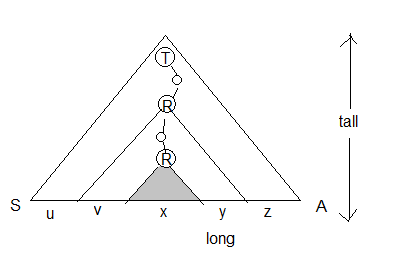
\includegraphics{5-2}
\end{center}

Look at the subtree that comes from the lower and upper instances of the repeated variable. Now let's make a ``surgery": take the subtree under the higher $R$ and stick it in place of the lower subtree. We now get another valid parse tree for $uvvxyyz$. We can repeat this as many times as we'd like.


\begin{center}
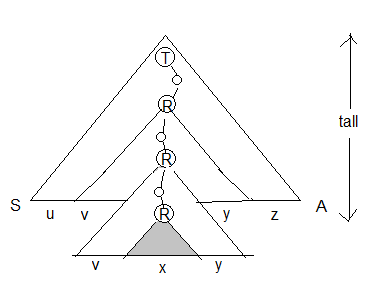
\includegraphics{5-3}
\end{center}


We get the $i=0$ case by sticking the lower tree on the upper $R$.

\begin{center}
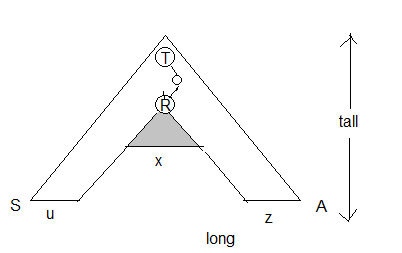
\includegraphics{5-3b}
\end{center}

There are some details to get the conditions to work.
\begin{itemize}
\item
How do we know that $v$ and $y$ are not both empty? If they are, we've shown nothing.

Let's start off with the parse tree with the {\it fewest} nodes. If $v$ and $y$ were both empty, then when we stick the lower $R$-subtree higher up as in the last picture above, we get fewer nodes, contradicting our minimality assumption. Hence $v$ and $y$ can't both be empty; this gives condition 2. 
\item
Let's figure out $p$. Let $b$ be the size of the largest right-hand side of a rule. We want the tallness to be at least $|V|+1$ ($|V|$ is the number of variables.) At each level, the number of nodes multiplies by at most $b$. If we set $p=b^{|V|+1}$, then the tree would have at least $|V|+1$ levels, so one of the symbols would repeat, as needed.
\item
To satisfy item 3 we take the lowest repetition of a symbol, so that there can be no repetitions below. This will give the bound $|vxy|\le p$.
\end{itemize}







\end{proof}

\subsection{Turing machines}

Everything we've done so far is a warm-up. We've given two models of computations that are deficient in a certain sense because they can't even do what we think computers can do, such as test whethere a string is of the form $a^kb^kc^k$.

A Turing machine is vastly more powerful; it is a much closer model to what we think about when we think about a general-purpose computer.

The input tape of a Turing machine combines the features of both the input and stack. It is a place where we can both read and write. 
\begin{itemize}
\item
We can read and write on the tape.
\end{itemize}
This is the key difference. The following are other differences.

\ig{5-5}{1}

\begin{itemize}
\item
We are able to both move the tape forward and back, so we can read what we wrote before. (It's a two way head.)
\item
The tape is infinite to the right. At the beginning, it is filled with a finite string, and the rest of the tape is filled will special symbols called blanks. The head starts on the leftmost tape cell.
\item The machine accepts by entering an ``accept" state anywhere. (It no longer makes sense to say the Turing machine accepts only at the end of the string---it might have erased or changed the last symbol!)
\item There is a ``reject" state; if the machine visits that state, stop and reject (reject by halting).
\item A Turing machine can also reject by entering an infinite loop (``looping").\footnote{How does the Turing machine know it has entered a infinite loop? Mathematically being able to define when the machine rejects is different from what we can tell from the machine's operation. We'll talk more about this later.}
%reject by entering a reject state, or by entering an infnite loop.
\end{itemize}
For the time being we'll just allow the deterministic variant.

\begin{ex}
We outline how to build a Turing machine that recognizes $\{a^nb^nc^n\}$.

Let's assume we can test when we're at the beginning. We go through the  string and cross out the first $a$, $b$, and $c$ that appear.

\ig{5-6}{1}

If we find letters that are out of order, we reject. Otherwise we go back to the beginning and continue to cross off symbols $a$, $b$, and $c$ one at a time. If we cross out the last $a$, $b$, and $c$ on the same run, then accept.

When we cross a symbol off, write the symbol $x$ to remember that we crossed out something there. %We have a tape alphabet.
\end{ex}
We'll write down the formal definition next time. Our transition function will depends on on both the state and tape symbol.
%qtikz